\definecolor{conv_lightgreen}{HTML}{bdddbd}
\definecolor{conv_darkgreen}{HTML}{8dbd8d}
\definecolor{conv_lightred}{HTML}{cdcddd}
\definecolor{conv_darkred}{HTML}{9d9dbd}

\newcommand{\filtersize}{3}
\newcommand{\filterx}{8}
\newcommand{\filtery}{2.2}
\newcommand{\filteroffset}{1}

\newcommand{\filterxres}{12}

\newcommand{\imagesize}{7}
\newcommand{\imagex}{0}
\newcommand{\imagey}{0}
\newcommand{\imageoffset}{2}

\newcommand{\outx}{12}
\newcommand{\outy}{0}
\newcommand{\outoffset}{2}

\newcommand{\percx}{1}
\newcommand{\percy}{2}
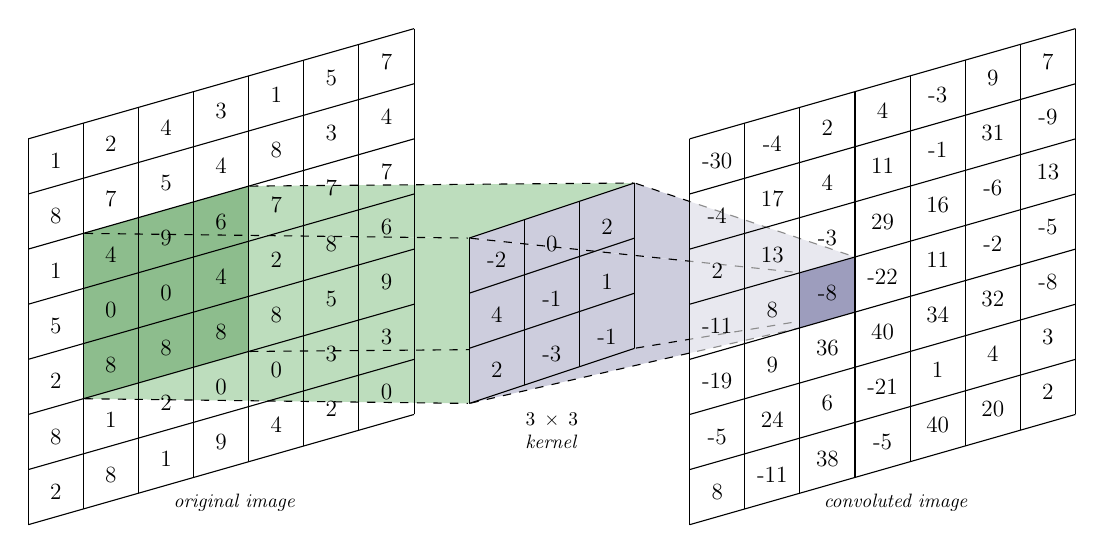
\begin{tikzpicture}[scale=0.7, every node/.style={transform shape}]
    \tikzstyle{point}=[draw=none,inner sep=0pt]

    % corner points of perceptive field
    \node (p1)[point] at (\imagex+\percx, \imagey+\percy+\percx*\imageoffset/\imagesize) {};
    \node (p2)[point] at (\imagex+\percx+\filtersize, \imagey+\percy+\percx*\imageoffset/\imagesize+\filtersize*\imageoffset/\imagesize) {};
    \node (p3)[point] at (\imagex+\percx+\filtersize, \imagey+\percy+\filtersize+\percx*\imageoffset/\imagesize+\filtersize*\imageoffset/\imagesize) {};
    \node (p4)[point] at (\imagex+\percx, \imagey+\percy+\filtersize+\percx*\imageoffset/\imagesize) {};

    % corner points of filter
    \node (f1)[point] at (\filterx, \filtery) {};
    \node (f2)[point] at (\filterx+3, \filtery+1) {};
    \node (f3)[point] at (\filterx+3, \filtery+4) {};
    \node (f4)[point] at (\filterx, \filtery+3) {};

    % corner points of output point
    \node (o1)[point] at (\outx+\percx+1, \outy+\percy+\percx*\outoffset/\imagesize+1+1*\outoffset/\imagesize) {};
    \node (o2)[point] at (\outx+\percx+2, \outy+\percy+\percx*\outoffset/\imagesize+1*\outoffset/\imagesize+1+1*\outoffset/\imagesize) {};
    \node (o3)[point] at (\outx+\percx+2, \outy+\percy+1+\percx*\outoffset/\imagesize+1*\outoffset/\imagesize+1+1*\outoffset/\imagesize) {};
    \node (o4)[point] at (\outx+\percx+1, \outy+\percy+2+\percx*\outoffset/\imagesize+1*\outoffset/\imagesize) {};

    % corner points of output image
    \node (op1)[point] at (\outx, \outy) {};
    \node (op2)[point] at (\outx+\imagesize, \outy+\outoffset) {};
    \node (op3)[point] at (\outx+\imagesize, \outy+\imagesize+\outoffset) {};
    \node (op4)[point] at (\outx, \outy+\imagesize) {};

    % draw image to filter shadow
    \fill[conv_lightgreen] (p1.center) -- (f1.center) -- (f4.center) -- (p4.center) -- (p1.center);
    \fill[conv_lightgreen] (f4.center) -- (f3.center) -- (p3.center) -- (p4.center) -- (f4.center);

    % draw perceptive field
    \fill[conv_darkgreen] (p1.center) -- (p2.center) -- (p3.center) -- (p4.center) -- (p1.center);

    % draw dashed connections image to filter
    \draw[dashed] (p1) -- (f1);
    \draw[dashed] (p2) -- (f2);
    \draw[dashed] (p3) -- (f3);
    \draw[dashed] (p4) -- (f4);

    % hide dashed lines behind filter
    \fill[white] (f1.center) -- (f2.center) -- (f3.center) -- (f4.center) -- (f1.center);

    % filter to output point
    \fill[conv_lightred] (f1.center) -- (o1.center) -- (o4.center) -- (f4.center) -- (f1.center);
    \fill[conv_lightred] (f4.center) -- (o4.center) -- (o3.center) -- (f3.center) -- (f4.center);

    % draw dashed connections filter to out
    \draw[dashed] (f1) -- (o1);
    \draw[dashed] (f2) -- (o2);
    \draw[dashed] (f3) -- (o3);
    \draw[dashed] (f4) -- (o4);

    % white overlay for output
    \fill[white, fill opacity=0.55] (op1.center) -- (op2.center) -- (op3.center) -- (op4.center) -- (op1.center);

    % draw output point
    \fill[conv_darkred] (o1.center) -- (o2.center) -- (o3.center) -- (o4.center) -- (o1.center);

    % draw image
    \foreach \x in {0,...,\imagesize}
    {
    \draw (\imagex+\x, \imagey+\x*\imageoffset/\imagesize) -- (\imagex+\x, \imagey+\imagesize+\x*\imageoffset/\imagesize);
    \draw (\imagex, \imagey+\x) -- (\imagex+\imagesize, \imagey+\x+\imageoffset);
    }

    % draw filter
    \foreach \x in {0,...,\filtersize}
    {
    \draw (\filterx+\x, \filtery+\x*\filteroffset/\filtersize) -- (\filterx+\x, \filtery+\filtersize+\x*\filteroffset/\filtersize);
    \draw (\filterx, \filtery+\x) -- (\filterx+\filtersize, \filtery+\x+\filteroffset);
    }

    % draw out
    \foreach \x in {0,...,\imagesize}
    {
    \draw (\outx+\x, \outy+\x*\outoffset/\imagesize) -- (\outx+\x, \outy+\imagesize+\x*\outoffset/\imagesize);
    \draw (\outx, \outy+\x) -- (\outx+\imagesize, \outy+\x+\outoffset);
    }

    \node at (\imagex + \imagesize/2 + 0.25,\imagey+0.4) {\emph{original image}};
     \node[text width=4cm, align=center] at (\filterx + \filtersize/2,\filtery + \filtersize - 3.5) {\emph{$3\times 3$\\kernel}};
    \node at (\outx + \imagesize/2 + 0.25,\outy+0.4) {\emph{convoluted image}};

    % Start image (left to right, top to bottom)
    \node[draw=none] at (0.5, 6.6) {\large 1};
    \node[draw=none] at (1.5, 6.9) {\large 2};
    \node[draw=none] at (2.5, 7.2) {\large 4};
    \node[draw=none] at (3.5, 7.5) {\large 3};
    \node[draw=none] at (4.5, 7.8) {\large  1};
    \node[draw=none] at (5.5, 8.1) {\large  5};
    \node[draw=none] at (6.5, 8.4) {\large  7};%%%%%%%%%%%%%%%%%%%%%%%%%%%%%%%

    \node[draw=none] at (0.5, 5.6) {\large 8};
    \node[draw=none] at (1.5, 5.9) {\large  7};
    \node[draw=none] at (2.5, 6.2) {\large 5};
    \node[draw=none] at (3.5, 6.5) {\large 4};
    \node[draw=none] at (4.5, 6.8) {\large 8};
    \node[draw=none] at (5.5, 7.1) {\large 3};
    \node[draw=none] at (6.5, 7.4) {\large  4};%%%%%%%%%%%%%%%%%%%%%%%%%%%%%%%

    \node[draw=none] at (0.5, 4.6) {\large 1};
    \node[draw=none] at (1.5, 4.9) {\large 4};
    \node[draw=none] at (2.5, 5.2) {\large 9};
    \node[draw=none] at (3.5, 5.5) {\large 6};
    \node[draw=none] at (4.5, 5.8) {\large  7};
    \node[draw=none] at (5.5, 6.1) {\large  7};
    \node[draw=none] at (6.5, 6.4) {\large 7};%%%%%%%%%%%%%%%%%%%%%%%%%%%%%%%

    \node[draw=none] at (0.5, 3.6) {\large 5};
    \node[draw=none] at (1.5, 3.9) {\large  0};
    \node[draw=none] at (2.5, 4.2) {\large 0};
    \node[draw=none] at (3.5, 4.5) {\large  4};
    \node[draw=none] at (4.5, 4.8) {\large 2};
    \node[draw=none] at (5.5, 5.1) {\large 8};
    \node[draw=none] at (6.5, 5.4) {\large 6};%%%%%%%%%%%%%%%%%%%%%%%%%%%%%%%

    \node[draw=none] at (0.5, 2.6) {\large 2};
    \node[draw=none] at (1.5, 2.9) {\large  8};
    \node[draw=none] at (2.5, 3.2) {\large  8};
    \node[draw=none] at (3.5, 3.5) {\large  8};
    \node[draw=none] at (4.5, 3.8) {\large 8};
    \node[draw=none] at (5.5, 4.1) {\large  5};
    \node[draw=none] at (6.5, 4.4) {\large  9};%%%%%%%%%%%%%%%%%%%%%%%%%%%%%%%

    \node[draw=none] at (0.5, 1.6) {\large 8};
    \node[draw=none] at (1.5, 1.9) {\large  1};
    \node[draw=none] at (2.5, 2.2) {\large  2};
    \node[draw=none] at (3.5, 2.5) {\large 0};
    \node[draw=none] at (4.5, 2.8) {\large  0};
    \node[draw=none] at (5.5, 3.1) {\large 3};
    \node[draw=none] at (6.5, 3.4) {\large 3};%%%%%%%%%%%%%%%%%%%%%%%%%%%%%%%

    \node[draw=none] at (0.5, 0.6) {\large 2};
    \node[draw=none] at (1.5, 0.9) {\large  8};
    \node[draw=none] at (2.5, 1.2) {\large 1};
    \node[draw=none] at (3.5, 1.5) {\large  9};
    \node[draw=none] at (4.5, 1.8) {\large  4};
    \node[draw=none] at (5.5, 2.1) {\large  2};
    \node[draw=none] at (6.5, 2.4) {\large  0};%%%%%%%%%%%%%%%%%%%%%%%%%%%%%%%

    % Filter
    \node[draw=none] at ( 8.5, 4.8) {\large  -2};
    \node[draw=none] at ( 9.5, 5.1) {\large 0};
    \node[draw=none] at (10.5, 5.4) {\large 2};%%%%%%%%%%%%%%%%%%%%%%%%%%%%%%%
    \node[draw=none] at ( 8.5, 3.8) {\large 4};
    \node[draw=none] at ( 9.5, 4.1) {\large  -1};
    \node[draw=none] at (10.5, 4.4) {\large  1};%%%%%%%%%%%%%%%%%%%%%%%%%%%%%%%
    \node[draw=none] at ( 8.5, 2.8) {\large  2};
    \node[draw=none] at ( 9.5, 3.1) {\large -3};
    \node[draw=none] at (10.5, 3.4) {\large  -1};%%%%%%%%%%%%%%%%%%%%%%%%%%%%%%%

    % Result image (left to right, top to bottom)
    % [[ -30	-4	2	4	-3	9	7]
    \node[draw=none] at (12.5, 6.6) {\large -30};
    \node[draw=none] at (13.5, 6.9) {\large -4};
    \node[draw=none] at (14.5, 7.2) {\large 2};
    \node[draw=none] at (15.5, 7.5) {\large 4};
    \node[draw=none] at (16.5, 7.8) {\large -3};
    \node[draw=none] at (17.5, 8.1) {\large 9};
    \node[draw=none] at (18.5, 8.4) {\large 7};%%%%%%%%%%%%%%%%%%%%%%%%%%%%%%%
    %  [-4	17	4	11	-1	31	-9]
    \node[draw=none] at (12.5, 5.6) {\large -4};
    \node[draw=none] at (13.5, 5.9) {\large  17};
    \node[draw=none] at (14.5, 6.2) {\large 4};
    \node[draw=none] at (15.5, 6.5) {\large 11};
    \node[draw=none] at (16.5, 6.8) {\large -1};
    \node[draw=none] at (17.5, 7.1) {\large 31};
    \node[draw=none] at (18.5, 7.4) {\large -9};%%%%%%%%%%%%%%%%%%%%%%%%%%%%%%%
    %  [2	13	3	29	16	-6	13]
    \node[draw=none] at (12.5, 4.6) {\large 2};
    \node[draw=none] at (13.5, 4.9) {\large  13};
    \node[draw=none] at (14.5, 5.2) {\large -3};
    \node[draw=none] at (15.5, 5.5) {\large  29};
    \node[draw=none] at (16.5, 5.8) {\large 16};
    \node[draw=none] at (17.5, 6.1) {\large -6};
    \node[draw=none] at (18.5, 6.4) {\large  13};%%%%%%%%%%%%%%%%%%%%%%%%%%%%%%%
    %  [-11	8	-8	-22	11	-2	-5]
    \node[draw=none] at (12.5, 3.6) {\large -11};
    \node[draw=none] at (13.5, 3.9) {\large  8};
    \node[draw=none] at (14.5, 4.2) {\large  -8};
    \node[draw=none] at (15.5, 4.5) {\large  -22};
    \node[draw=none] at (16.5, 4.8) {\large  11};
    \node[draw=none] at (17.5, 5.1) {\large  -2};
    \node[draw=none] at (18.5, 5.4) {\large -5};%%%%%%%%%%%%%%%%%%%%%%%%%%%%%%%
    %  [-19	9	36	40	34	32	-8]
    \node[draw=none] at (12.5, 2.6) {\large -19};
    \node[draw=none] at (13.5, 2.9) {\large  9};
    \node[draw=none] at (14.5, 3.2) {\large  36};
    \node[draw=none] at (15.5, 3.5) {\large   40};
    \node[draw=none] at (16.5, 3.8) {\large  34};
    \node[draw=none] at (17.5, 4.1) {\large 32};
    \node[draw=none] at (18.5, 4.4) {\large   -8};%%%%%%%%%%%%%%%%%%%%%%%%%%%%%%%
    %  [-5	24	6	-21	1	4	3]
    \node[draw=none] at (12.5, 1.6) {\large -5};
    \node[draw=none] at (13.5, 1.9) {\large  24};
    \node[draw=none] at (14.5, 2.2) {\large 6};
    \node[draw=none] at (15.5, 2.5) {\large  -21};
    \node[draw=none] at (16.5, 2.8) {\large   1};
    \node[draw=none] at (17.5, 3.1) {\large  4};
    \node[draw=none] at (18.5, 3.4) {\large  3};%%%%%%%%%%%%%%%%%%%%%%%%%%%%%%%
    %  [ 8	-11	38	-5	40	20	2]]
    \node[draw=none] at (12.5, 0.6) {\large 8};
    \node[draw=none] at (13.5, 0.9) {\large -11};
    \node[draw=none] at (14.5, 1.2) {\large 38};
    \node[draw=none] at (15.5, 1.5) {\large -5};
    \node[draw=none] at (16.5, 1.8) {\large 40};
    \node[draw=none] at (17.5, 2.1) {\large  20};
    \node[draw=none] at (18.5, 2.4) {\large 2};%%%%%%%%%%%%%%%%%%%%%%%%%%%%%%%
\end{tikzpicture}